%%%%%%%%%%%%%%%%%%%%%%%%%%%%%
% Standard header for working papers
%
% WPHeader.tex
%
%%%%%%%%%%%%%%%%%%%%%%%%%%%%%

\documentclass[11pt]{article}

%%%%%%%%%%%%%%%%%%%%
%% Include general header where common packages are defined
%%%%%%%%%%%%%%%%%%%%

% general packages without options
\usepackage{amsmath,amssymb,bbm}




%%%%%%%%%%%%%%%%%%%%
%% Idem general commands
%%%%%%%%%%%%%%%%%%%%
%% Commands

\newcommand{\noun}[1]{\textsc{#1}}


%% Math

% Operators
\DeclareMathOperator{\Cov}{Cov}
\DeclareMathOperator{\Var}{Var}
\DeclareMathOperator{\E}{\mathbb{E}}
\DeclareMathOperator{\Proba}{\mathbb{P}}

\newcommand{\Covb}[2]{\ensuremath{\Cov\!\left[#1,#2\right]}}
\newcommand{\Eb}[1]{\ensuremath{\E\!\left[#1\right]}}
\newcommand{\Pb}[1]{\ensuremath{\Proba\!\left[#1\right]}}
\newcommand{\Varb}[1]{\ensuremath{\Var\!\left[#1\right]}}

% norm
\newcommand{\norm}[1]{\| #1 \|}


% amsthm environments
\newtheorem{definition}{Definition}



%% graphics

% renew graphics command for relative path providment only ?
%\renewcommand{\includegraphics[]{}}








% geometry
\usepackage[margin=2cm]{geometry}

% layout : use fancyhdr package
\usepackage{fancyhdr}
\pagestyle{fancy}

\makeatletter

\renewcommand{\headrulewidth}{0.4pt}
\renewcommand{\footrulewidth}{0.4pt}
%\fancyhead[RO,RE]{\textit{Working Paper}}
\fancyhead[RO,RE]{\textit{ECTQG 2015}}
%\fancyhead[LO,LE]{G{\'e}ographie-Cit{\'e}s/LVMT}
\fancyhead[LO,LE]{An Algorithmic Systematic Review}
\fancyfoot[RO,RE] {\thepage}
\fancyfoot[LO,LE] {\noun{J. Raimbault}}
\fancyfoot[CO,CE] {}

\makeatother


%%%%%%%%%%%%%%%%%%%%%
%% Begin doc
%%%%%%%%%%%%%%%%%%%%%

\begin{document}







\title{Sensitivity of Urban Scaling Exponents to City Definition\bigskip\\
\textit{Working Paper}
}
\author{\noun{Juste Raimbault}}
\date{Tuesday 19th May}


\maketitle

\justify


\begin{abstract}
Scaling laws have been shown to be universal of urban systems at many scales and for many indicators. Recent studies question however the consistence of scaling exponents determination, as their value can vary significantly depending on thresholds used to define urban entities on which quantities are integrated, even crossing the qualitative border of linear scaling, from infralinear to supralinear scaling. We use a simple theoretical model of spatial distribution of densities and urban functions to show analytically that such behavior can be derived as a consequence of the type of spatial distribution and the method used. Numerical simulation confirm the theoretical results and reveals that results are reasonably independant of spatial kernel used to distribute density.
\end{abstract}


%%%%%%%%%%%%%%%%%%%%
\section{Introduction}

Scaling laws for urban systems, starting from the well-known rank-size Zipf's law for city size distribution~\cite{gabaix1999zipf}, have been shown to be a recurrent feature of urban systems, at many scales and for many types of indicators. They reside in the empirical constatation that indicators computed on elements of an urban system, that can be cities for system of cities, but also smaller entities at a smaller scale, do fit relatively well a power-law distribution as a function of entity size, i.e. that for entity $i$ with population $P_i$, we have for an integrated quantity $A_i$, the relation $A_i \simeq A_0\cdot \left(\frac{P_i}{P_0}\right)^{\alpha}$. Scaling exponent $\alpha$ can be smaller or greater than 1, leading to infra- or supralinear effects. Various thematic interpretation of this phenomena have been proposed, typically under the form of processes analysis. The economic literature has produced abundant work on the subject (see~\cite{Gabaix20042341} for a review), but that are generally poorly spatialized, thus of poor interest to our approach that deals precisely with spatial organization. Simple economic rules such as energetic equilibria can lead to simple power-laws~\cite{bettencourt2008large} but are difficult to fit empirically. A interesting proposition by Pumain is that they are intrinsically due to the evolutionnary character of city systems, where complex emergent interaction between cities generate such global distributions~\cite{pumain2006evolutionary}. Although a tempting parallel can be done with self-organizing biological systems, Pumain insists on the fact that the ergodicity assumption for such systems is not reasonable in the case of geographical systems and that the analogy cannot be exploited~\cite{pumain2012urban}. Other explanations have been proposed at other scales, such as the urban growth model at the mesoscopic scale (city scale) given in~\cite{2014arXiv1401.8200L} that shows that the congestion within transportation networks may be one reason for city shapes and corresponding scaling laws. Note that ``classic'' urban growth models such as Gibrat's model do provide first order approximation of scaling systems, but that interactions between agaents have to be incorporated into the model to obtain better fit on real data, such as the Favaro-Pumain model for innovation cycles propagation proposed in~\cite{favaro2011gibrat}, that generalize a Gibrat model and provide better fits on data for French cities.

However, the blind application of scaling exponents computations was recently pointed as misleading in most cases~\cite{louf2014scaling}, confirmed by empirical works such as~\cite{2013arXiv1301.1674A} that showed the variability of computed exponents to the parameters defining urban areas, such as density thresholds. An ongoing work by Cottineau \& \textit{al.} presented at~\cite{cottineau2015scaling}, studies empirically for French Cities the influence of 3 parameters playing a role in city definition, that are a density threshold $\theta$ to delimitate boundaries of an urban area, a number of commuters threshold $\theta_c$ that is the proportion of commuters going to core area over which the unity is considered belonging to the area, and a cut-off parameter $P_c$ under which entities are not taken into account for the linear regression providing the scaling exponent. Remarquable results are that exponents can significantly vary and move from infralinear to supralinear when threshold varies. A systematic exploration of parameter space produces phase diagrams of exponents for various quantities. One question raising immediately is how these variation can be explained by the features of spatial distribution of variables. Do they result from intrinsic mechanisms present in the system or can they be explained more simply by the fact that the system is particularly spatialized ? We propose to prove by the tractation of a toy analytical model that even simple distributions can lead to such significant variations in the exponents, along one dimension of parameters (density threshold), directing the response towards the second explanation. The rest of the paper is organized as follows : we formalize the simple framework used and derive an analytical relation between estimated exponent and density threshold parameter. We then present a numerical implementation of the model that confirms numerically theoretical results, explore other form of kernels that would be less tractable, and study the sensitivity along two parameters. We finally discuss the implications of our results and further work needed.

%%%%%%%%%%%%%%%%%%%%
\section{Formalization}
\label{sec:formalization}

We formalize the simple theoretical context in which we will derive the sensitivity of scaling to city definition. Let consider a polycentric city system, which spatial density distributions can be reasonably constructed as the superposition of monocentric fast-decreasing spatial kernels, such as an exponential mixture model~\cite{anas1998urban}. Taking a geographical space as $\mathbb{R}^2$, we take for any $\vec{x}\in\mathbb{R}^2$ the density of population as
\begin{equation}
d(\vec{x}) = \sum_{i=1}^{N}{d_i(\vec{x})} = \sum_{i=1}^{N}{d_i^0\cdot \exp{\left(\frac{-\norm{\vec{x}-\vec{x}_i}}{r_i}\right)}}
\end{equation}

where $r_i$ are spread parameters of kernels, $d_i^0$ densities at origins, $\vec{x}_i$ positions of centers. We furthemore assume the following constraints :

\begin{enumerate}
\item To simplify, cities are monocentric, in the sense that for all $i\neq j$, we have $\norm{\vec{x}_i - \vec{x}_j}\gg r_i$.
\item It allows to impose structural scaling in the urban system by the simple constraint on city populations $P_i$. One can compute by integration that $P_i=2\pi d_i^0 r_i^2$, what gives by injection into the scaling hypothesis $\ln{P_i}=\ln{P_{max}}-\alpha \ln{i}$, the following relation between parameters : $\ln{\left[d_i^0 r_i^2\right]}=K' - \alpha \ln{i}$.
\end{enumerate}

To study scaling relations, we consider a random scalar spatial variable $a(\vec{x})$ representing one aspect of the city, that can be everything but has the dimension of a spatial density, such that the indicator $A(D)=\Eb{\iint_D{a(\vec{x})d\vec{x}}}$ represents the expected quantity of $a$ in area $D$. We make the assumption that $a\in \{0;1\}$ (``counting'' indicator) and that its law is given by $\Pb{a(\vec{x})=1}=f(d(\vec{x}))$. Following the empirical work done in~\cite{cottineau2015scaling}, the integrated indicator on city $i$ as a function of $\theta$ is given by
\[
A_i(\theta) = A(D(\vec{x}_i, \theta))
\]

where $D(\vec{x}_i, \theta)$ is the area centered in $\vec{x}_i$ where $d(\vec{x})>\theta$. Assumption 1 ensures that the area are roughly disjoint circles. We take furthermore a simple amenity such that it follows a local scaling law in the sense that $f(d)=\lambda\cdot d^\beta$. It seems a reasonable assumption since it was shown that many urban variable follow a fractal behavior at the intra-urban scale~\cite{keersmaecker2003using} and that it implies necessarily a power-law distribution~\cite{chen2010characterizing}. We make the additional assumption that $r_i=r_0$ does not depend on $i$, what is reasonable if the urban system is considered from a large scale. This assumption should be relaxed in numerical simulations. The estimated scaling exponent $\alpha(\theta)$ is then the result of the log-regression of $(A_i(\theta))_i$ against $(P_i(\theta))_i$ where $P_i(\theta)=\iint_{D(\vec{x}_i,\theta)}{d}$.


%%%%%%%%%%%%%%%%%%%%
\section{Analytical Derivation of Sensitivity}

With above notations, let derive the expression of estimated exponent for quantity $a$ as a function of density threshold parameter $\theta$. The quantity computed for a given city $i$ is, thanks to the monocentric assumption and in a spatial range and a range for $\theta$ such that $\theta \gg \sum_{j\neq i}{d_j(\vec{x})}$, allowing to approximate $d(\vec{x})\simeq d_i(\vec{x})$ on $D(\vec{x}_i,\theta)$, is computed by
\[
\begin{split}
A_i(\theta) & = \lambda\cdot \iint_{D(\vec{x}_i,\theta)}{d^\beta} = 2\pi\lambda {d_i^0}^{\beta} \int_{r=0}^{r_0 \ln{\frac{d_i^0}{\theta}}}{r\exp{\left(-\frac{r\beta}{r_0}\right)}dr}\\
& = \frac{2\pi {d_i^0}^\beta r_0^2}{\beta^2} \left[1 + \beta \ln{\frac{\theta}{d_i^0}\left(\frac{\theta}{d_i^0}\right)^\beta} - \left(\frac{\theta}{d_i^0}\right)^\beta\right]
\end{split}
\]

We obtain in a similar way the expression of $P_i(\theta)$
\[
P_i(\theta) = 2\pi d_i^0 r_0^2 \left[1 + \ln{\left[\frac{\theta}{d_i^0}\right]}\frac{\theta}{d_i^0} - \frac{\theta}{d_i^0}\right]
\]

The Ordinary-Least-Square estimation, solving the problem $\inf_{\alpha,C}\norm{(\ln{A_i(\theta)} - C - \alpha \ln{P_i(\theta)})_i}^2$, gives the value $\alpha(\theta) = \frac{\Covb{(\ln{A_i(\theta)})_i}{(\ln{P_i(\theta)})_i}}{\Varb{(\ln{P_i(\theta)})_i}}$. As we work on city boundaries, threshold is expected to be significantly smaller than center density, i.e. $\theta / d_i^0 \ll 1$. We can develop the expression in the first order of $\theta / d_i^0$ and use the global scaling law for city sizes, what gives $\ln{A_i(\theta)} \simeq K_A - \alpha \ln{i} + (\beta - 1)\ln{d_i^0} + \beta \ln{\frac{\theta}{d_i^0}\left(\frac{\theta}{d_i^0}\right)^\beta} $ and $\ln{P_i(\theta)} = K_P - \alpha \ln{i} + \ln{\left[\frac{\theta}{d_i^0}\right]}\frac{\theta}{d_i^0}$. Developping the covariance and variance gives finally an expression of the scaling exponent as a function of $\theta$, where $k_j,{k_j}'$ are constants obtained in the development :

\begin{equation}
\label{eq:th}
\alpha(\theta) = \frac{k_0 + k_1 \theta + k_2 \theta^\beta + k_3 \theta^{\beta + 1} +  k_4 \theta \ln{\theta} + k_5 \theta^\beta \ln{\theta} + k_6 \theta^\beta (\ln{\theta})^2 + k_7 \theta^{\beta + 1}(\ln{\theta})^2 + k_8 \theta^{\beta + 1}\ln{\theta}}{k_0'+k_1' \ln{\theta} + k_2' \theta \ln{\theta} + k_3' \theta^2 + k_4' \theta^2\ln{\theta} + k_5' \theta^2 (\ln{\theta})^2}
\end{equation}

This rational fraction predicts the evolution of the scaling exponent when the threshold varies. We study numerically its behavior in the next section, among other numerical experiments.


%%%%%%%%%%%%%%%%%%%%
\section{Numerical Simulations}

\paragraph{Implementation}

We implement empirically the density model given in section~\ref{sec:formalization}. Centers are successively chosen such that in a given region of space only one kernel dominates in the sense that the sum of other contributions are above a given threshold $\theta_e$. In practice, adapting $N$ to world size allows to respect the monocentric condition. Population are distributed in order to follow the scaling law with fixed $\alpha$ and $r_i$ (arbitrary choice) by computing corresponding $d_i^0$. Technical details of the implementation done in R~\cite{R-Core-Team:2015fk} and using the package \texttt{kernlab} for efficient kernel mixture methods~\cite{Karatzoglou:2004uq} are given as comments in source code\footnote{available at \texttt{https://github.com/JusteRaimbault/CityNetwork/tree/master/Models/Scaling}}. We show in figure~\ref{fig:ex-distrib} example of synthetic density distributions on which the numerical study is conducted. Theoretical result obtained in Eq.~\ref{eq:th} are studied and confronted to emprically computed values for various parameter as shown in Fig.~\ref{fig:th_results}.

\begin{figure}
\centering
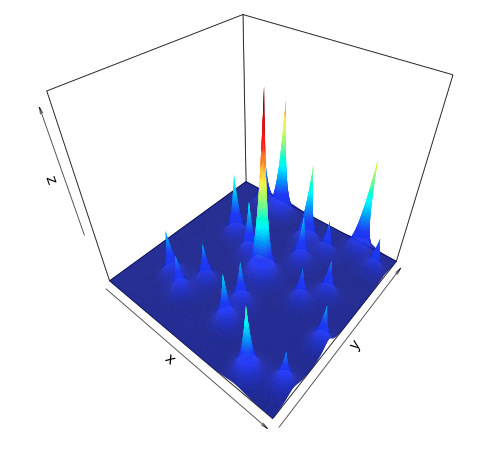
\includegraphics[width=0.4\textwidth]{figures/example_exp_mixture}
\caption{Example of a synthetic density distribution obtained with the exponential mixture, with a grid of size $400\times 400$ and parameters $N=20$, $r_0=10$, $P_{max}=200$, $\alpha=0.5$, $\theta_C = 0.01$.}
\label{fig:ex-distrib}
\end{figure}


\begin{figure}
\centering

\caption{Validation of theoretical result through numerical simulation.}
\label{fig:th_results}
\end{figure}



\paragraph{Random Perturbations}

The simple model used is quite reducing for maximal densities and radius distribution. We proceed to an empirical study of the influence of noise in the system by fixing $d_i^0$ and $r_i$ the following way :
\begin{itemize}
\item $d_i^0$ follows a reversed log-normal distribution with maximal value being a realistic maximal density
\item Radiuses are computed to respect rank-size law and then perturbated by a white noise.
\end{itemize}

Results shown in Fig.~\ref{fig:random-density} are quantitatively different from previous one, as expected, but the same qualitative behavior is reproduced.


\begin{figure}
\centering

\caption{Variation of exponents with variable origin density and radius.}
\label{fig:random-density}
\end{figure}



\paragraph{Kernel Type}

We test the influence of the type of spatial kernel used on results. We test gaussian kernels and quadratic kernels with parameters within reasonable ranges analog to the exponential kernel. As shown in Fig.~\ref{fig:other-kernels}, we obtain the same qualitative results that is the significant variation of $\alpha(\theta)$ as a function of $\theta$.


%TODO
\begin{figure}
\centering

\caption{Scaling exponents for other kernels.}
\label{fig:other-kernels}
\end{figure}





\paragraph{Two-parameters phase diagram}

We introduce now a second spatial variable that has also an influence on the definition of urban entities, that is the proportion of actives working in city center, as done on empirical data in~\cite{cottineau2015scaling}. To simplify, it is used only to define urban parameter but assumed as having no influence on the local probability distribution of the amenity which stays the same function of the density. We write 


\begin{figure}
\centering

\caption{Two parameters phase diagram.}
\label{fig:two-params}
\end{figure}



%%%%%%%%%%%%%%%%%%%%
\section{Discussion}




%%%%%%%%%%%%%%%%%%%%
\section{Conclusion}






%%%%%%%%%%%%%%%%%%%%
%% Biblio
%%%%%%%%%%%%%%%%%%%%

\bibliographystyle{apalike}
\bibliography{/Users/Juste/Documents/ComplexSystems/CityNetwork/Biblio/Bibtex/CityNetwork}


\end{document}
